% $Author: Luc $
% $Date: 2008-11-09 11:14:31 +0200 (Sun, 09 Nov 2008) $
% $Revision:  $
%=================================================================
\ifx\wholebook\relax\else
% --------------------------------------------
% Lulu:
    \documentclass[a4paper,10pt,twoside]{book}
    \usepackage[
        papersize={6in,9in},
        hmargin={.75in,.75in},
        vmargin={.75in,1in},
        ignoreheadfoot
    ]{geometry}
    \input{../common.tex}
    \pagestyle{headings}
    \setboolean{lulu}{true}
% --------------------------------------------
% A4:
%   \documentclass[a4paper,11pt,twoside]{book}
%   \input{../common.tex}
%   \usepackage{a4wide}
% --------------------------------------------
    \graphicspath{{figures/} {../figures/}}
    \begin{document}
%   \renewcommand{\nnbb}[2]{} % Disable editorial comments
    \sloppy
\fi

\chapter{Variables}\label{cha:variables}

\noindent\hrule
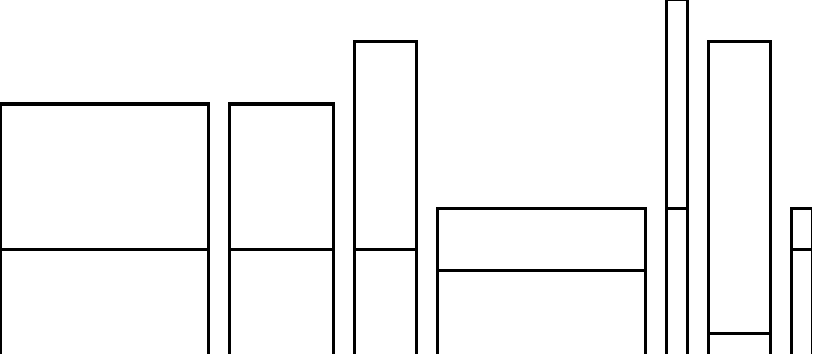
\includegraphics[width=0.9\linewidth]{varTitlePicture}
\noindent\hrule\vspace{1.5cm}

Les gens sont toujours en train de donner des noms aux choses. Par exemple, nous donnons des noms aux personnes, aux chiens et aux voitures. Lorsque nous faisons cela, nous \emph{associons} un objet, un \^etre, ou une id\'ee avec un mot ou un symbole. Une fois que cette association a \'et\'e faite, on peut alors utiliser le mot ou le symbole pour \emph{d\'esigner} ou d'interagir avec l'objet qui lui est associ\'e. Un nom peut durer toute une vie, ou il peut \^etre abandonn\'e apr\`es une courte p\'eriode. Parfois, les noms se r\'ef\`erent \`a d'autres noms. Par exemple, un acteur a g\'en\'eralement plusieurs noms: son vrai nom, un nom de sc\`ene, et le nom du personnage qu'il joue actuellement sur sc\`ene ou \`a l'\'ecran. Dans un langage de programmation, nous devons \'egalement \^etre capable de nommer les choses, et les \emph{variables} sont utilis\'ees \`a cette fin. 

Dans ce chapitre, vous apprendrez \`a utiliser les variables, qui sont des param\`etres substituables   pour les objets, et vous verrez comment les variables aident \`a simplifier les programmes. En effet, les variables sont souvent n\'ecessaires dans la programmation. Enfin, lorsque la complexit\'e des probl\`emes que vous rencontrez augmente, vous verrez que vous aurez besoin d'exprimer les d\'ependances entre les variables. Par exemple, la largeur d'un rectangle peut \^etre de deux-tiers sa longueur. Dans ce chapitre, je vais vous montrer comment utiliser les variables pour exprimer les d\'ependances entre les diff\'erentes quantit\'es. 

\section{Apport\'e \`a vous par la lettre A } 

Comme vous l'avez fait dans le chapitre~\ref{cha:robots}, supposons que vous souhaitez utiliser un robot pour \'ecrire des lettres de l'alphabet. La lettre A, plut\^ot primitive, que nous allons dessiner est caract\'eris\'ee par sa \emph{hauteur}, sa \emph{largeur}, et sa \emph{mi-hauteur} qui est la hauteur \`a laquelle la ligne m\'ediane de  A doit \^etre d\'essin\'ee, comme le montre la Figure~\ref{fig:varannotated}.. 

\begin{figure}
\center{\includegraphics[width=5cm]{varAnnotated}}
\caption{La forme de la lettre A est caract\'eris\'ee par sa hauteur, sa largeur et sa mi-hauteur. \label{fig:varannotated}}
\end{figure}

\begin{exonofig}\label{xp:anA100x70}
Ecrire un script qui dessine une lettre A de hauteur 100 pixels, de largeur 70 pixels, et de mi-hauteur 60 pixels. 
\end{exonofig}


\subsection{Variations sur le th\`eme de A} 

Le script que vous avez \'ecrit pour l'exp\'erience 8-1 devrait ressembler au script~\ref{scr:anA100x70}.  

\begin{script}[anA100x70]{Un A pour l'exp\'erience~\ref{xp:anA100x70}.}
| pica | 
pica := Bot new. 
pica north. 
pica go: 100. 
pica east. 
pica go: 70. 
pica south. 
pica go: 100. 
pica west. 
pica jump: 70. 
pica north. 
pica go: 60. 
pica east. 
pica go: 70 
\end{script}

\begin{exofigwithsizeandtitle}[0.7]{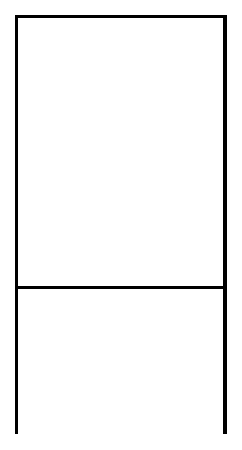
\includegraphics[width=2cm]{varA200}}{frAnkenstein}\label{xp:frankenstein}
Modifier le script~\ref{scr:anA100x70} pour dessiner une monstrueuse lettre A de  200 pixels de hauteur, de 100 pixels de largeur, et de 70 pixels de  mi-hauteur, comme le montre la figure ci-dessous. 
\end{exofigwithsizeandtitle}

En modifiant le script~\ref{scr:anA100x70} pour l'exp\'erience~\ref{xp:frankenstein}, vous avez trouv\'e que pour produire un A de taille diff\'erente, vous avez d\^u changer les nombres repr\'esentant la hauteur, la largeur, et la mi-hauteur de la lettre \emph{partout} o\`u ils se produisent et de mani\`ere  \emph{synchrone}.Par synchrone, je veux dire ``dans le bon ordre'', c'est \`a dire que 100 devrait devenir 200, 70 devrait devenir 100, et 60 devrait devenir 70 sans confusion. 

\begin{exonofigtitle}{Une vari\'et\'e de A}\label{xp:varietya}

Modifier le script~\ref{scr:anA100x70} pour dessiner d'autres A de diff\'erentes tailles que vous choisirez. Essayez de reproduire certains des A apparaissant dans l'image au d\'ebut de ce chapitre. 

\end{exonofigtitle}

En faisant l'exp\'erience~\ref{xp:varietya}, vous \^etes sans doute arriv\'e \`a la conclusion que modifier les valeurs des caract\'eristiques d'un A,  partout, est fastidieux. De plus, il devrait \^etre \'evident que, en r\'ealisant de tels changements, vous courez le risque de devenir confus ou d'oublier de changer une valeur ou d'apporter une modification \`a une valeur incorrecte. Le r\'esultat peut \^etre totalement diff\'erent de ce que vous aviez en t\^ete pour votre script. Vous pouvez imaginer que dans des programmes complexes, le changement des valeurs une par une de cette mani\`ere peut devenir tr\`es probl\'ematique. 

\section{Variables \`a la rescousse}

La r\'ealisation  d'un grand nombre de changements dans la production de lettres de diff\'erentes tailles et de diff\'erentes formes est \`a la fois fastidieux et source d'erreurs, et nous avons donc besoin d'une solution qui permettra \`a la fois de nous emp\^echer  de m\'elanger les nombres repr\'esentant les diff\'erentes caract\'eristiques d'une lettre et de nous permettre d'apporter des transformations sans avoir \`a changer toutes les valeurs partout o\`u elles se trouvent. En fait, nous aimerions \^etre capable de faire ce qui suit: 

\begin{itemize}
	\item \emph{D\'eclarer}  la hauteur, la largeur et la mi-hauteur d'une lettre A une seule fois pour l'ensemble du script.
	\item Se \emph{r\'ef\'erer} \`a ces valeurs si n\'ecessaire. 
	\item \emph{Changer} les valeurs si n\'ecessaire. 
\end{itemize}

Ces trois choses sont exactement ce qu'une variable nous permet de faire! Incroyable non? Une variable est un \emph{nom} auquel nous \emph{associons une valeur}. Nous devons la \emph{d\'eclarer} et l'\emph{associer} \`a une nouvelle valeur. Ensuite, nous pouvons nous \emph{r\'ef\'erer} \`a une variable et obtenir la \emph{valeur} qui lui est associ\'ee. Il est \'egalement possible de \emph{modifier} la valeur associ\'ee \`a une variable et de lui affecter une nouvelle valeur. La valeur d'une variable peut \^etre un nombre, une collection d'objets, ou m\^eme un robot. Nous allons maintenant illustrer comment d\'eclarer, associer une valeur, et utiliser une variable. 

\important{Important! Une variable est un \emph{nom} auquel on associe une \emph{valeur}. Nous d\'eclarons une variable et associons une valeur \`a elle. Ensuite, nous pouvons nous r\'ef\'erer \`a une variable et obtenir sa \emph{valeur}. Il est \'egalement possible de \emph{modifier} la valeur associ\'ee \`a une variable et de lui associer une nouvelle valeur.}

\subsection{D\'eclaration d'une variable } 

Avant d'utiliser une variable, nous devons la \emph{d\'eclarer}; c'est \`a dire, nous devons dire \`a Squeak le nom de la variable que nous voulons utiliser. Nous d\'eclarons des variables en les enfermant entre des barres verticales \ct{||}, comme le montre l'exemple suivant, qui d\'eclare les trois variables \ct{hauteur}, \ct{largeur}, et \ct{mi-hauteur}:

\ct{| hauteur largeur mi-hauteur |} 

Pour \^etre pr\'ecis, les barres verticales \ct{||} d\'eclarent des variables \emph{temporaires}, qui sont des variables qui n'existent que pendant l'ex\'ecution du script. 


\subsection{Affectation d'une valeur \`a une variable } 

Avant d'utiliser une variable, il est presque toujours n\'ecessaire de lui donner une valeur. Associer une valeur est appel\'e \emph{assigner} une valeur \`a une variable. En Smalltalk, la paire de symboles \ct{:=} est utilis\'e en association pour attribuer une valeur \`a une variable. Dans le script suivant, apr\`es avoir d\'eclar\'e trois variables, nous assignons $100$ \`a la variable \ct{hauteur}, $70$ \`a la variable  \ct{largeur}, et $60$ \`a la variable \ct{mi-hauteur}. Lorsque nous assignons une valeur \`a une variable pour la premi\`ere fois, nous disons que nous l'\emph{initialisons} : 

\begin{code}{}
| hauteur largeur mi-hauteur | 
hauteur := 100. 
largeur := 70. 
mi-hauteur := 60 
\end{code}

\important{Important! Le symbole \ct{:=} assigne une valeur \`a une variable. Par exemple,  \ct{hauteur := 120} assigne la valeur \ct{120} \`a la variable \ct{hauteur}, tandis que \ct{longueur := 120 + 30} assigne le r\'esultat de l'expression \ct{120 + 30}, c'est-\`a-dire \ct{150}, \`a la variable \ct{longueur}. 
}

Lorsque nous assignons une valeur \`a une variable pour la premi\`ere fois, nous disons que nous  l'\emph{initialisons}. 

\subsection{R\'ef\'erence \`a des variables } 

To refer to the value assigned to a variable---we also say \emph{use} a variable---simply write its name 
in a script. In the following script, after being \emph{declared} in line 1, the variable \ct{height} is \emph{initialized} with the value \ct{100} in line 3 and \emph{used} in line 5 to tell the created robot to go forward the number of pixels associated with the variable \ct{height}, which here is \ct{100}. 

Pour faire r\'ef\'erence \`a la valeur assign\'ee \`a une variable---on dit aussi \emph{utiliser} une variable---il suffit simplement d'\'ecrire son nom dans un script. Dans le script suivant, apr\`es avoir \'et\'e \emph{d\'eclar\'ee} \`a la ligne 1, la variable \ct{hauteur} est \emph{initialis\'ee} avec la valeur \ct{100} \`a la ligne 3 et \emph{utilis\'ee} \`a la ligne 5 pour dire au robot cr\'e\'e de se d\'eplacer vers l'avant du nombre de pixels associ\'e \`a la variable \ct{hauteur}, qui est ici \ct{100}. 

\begin{code}{}
| pica hauteur | 
pica := Bot new. 
hauteur := 100 
pica north. 
pica go: !\textbf{hauteur}!
\end{code}

\important{Important! En g\'en\'eral, une variable doit \^etre \emph{d\'eclar\'ee} et initialis\'ee avant d'\^etre utilis\'ee. }

\subsection{Et qu'en est-il de Pica? } 

Vous l'avez devin\'e! \ct{pica} est \'egalement une variable. Il se trouve \^etre une variable dont la valeur est un robot. Donc, \ct{| pica |} d\'eclare une variable nomm\'ee \ct{pica}. L'expression  \ct{pica := Bot new} initialise la variable avec une valeur, ici un nouveau robot. Ensuite, nous utilisons ce robot en lui envoyant des messages via la variable \ct{pica}, par exemple, \ct{pica go: 100}. 

\section{Utilisation des variables } 

Maintenant, explorons les avantages de l'utilisation des variables, et je vais vous montrer quelques propri\'et\'es puissantes que les variables poss\`edent. En particulier, je vais vous montrer la puissance provenant de l'expression de relations entre variables. 

En introduisant des variables dans Script~\ref{scr:anA100x70}, nous obtenons le script ~\ref{scr:anA100x70withvar}.


\begin{script}[anA100x70withvar]{Un A avec des variables.}
| pica !\textbf{hauteur largeur mi-hauteur}!| 
pica := Bot new. 
!\textbf{hauteur:= 100.}!              ``initialise les variables`` 
!\textbf{width:= 70.}! 
!\textbf{midheight:= 60.}! 
pica north. 
pica go: !\textbf{hauteur}!.            ``puis nous utilisons les variables`` 
pica east. 
pica go: !\textbf{largeur}!. 
pica south. 
pica go: !\textbf{hauteur}!. 
pica west. 
pica jump: !\textbf{largeur}!. 
pica north. 
pica go: !\textbf{mi-hauteur}!. 
pica east. 
pica go: !\textbf{largeur}! 
\end{script}

Vous serez d'accord que modifier les valeurs des variables est plus facile que de modifier des nombres dispers\'es dans tout le script. Changez quelques valeurs pour vous en convaincre. Vous devriez \^etre capable de dessiner tout les A apparaissant dans la figure au d\'ebut ce chapitre. Maintenant, si vous souhaitez modifier les caract\'eristiques de votre lettre A, il vous suffit seulement de r\'einitialiser les variables en modifiant les valeurs des lignes 3, 4 et 5, comme indiqu\'e dans le script~\ref{scr:anA100x70changevalues}. Le dessin obtenu est pr\'esent\'e dans la Figure~\ref{fig:varaflat}. 

\begin{script}[anA100x70changevalues]{Une lettre A modifi\'e}
| pica !\textbf{hauteur largeur mi-hauteur}! | 
pica := Bot new. 
!\textbf{hauteur:= 30.}!       ``initialise the variables`` 
!\textbf{largeur:= 200.}! 
!\textbf{mi-hauteur:= 10.}! 
... 
\end{script}


\begin{figure}[h!]
\centering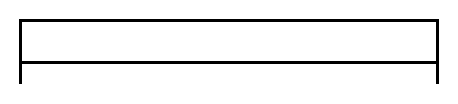
\includegraphics[width=5cm]{varAFlat}
\caption{Une petite et \'epaisse lettre A tout simplement cr\'e\'e avec hauteur = 30, largeur = 200, et mi-hauteur = 10.\label{fig:varaflat}}
\end{figure}

En utilisant des variables, vous pouvez facilement cr\'eer de nombreuses lettres diff\'erentes, et dans le futur, vous serez en mesure d'\'ecrire des programmes pour r\'esoudre de nombreux probl\`emes difficiles. Prenons du recul pour un moment et consid\'erons la puissance fournie par les variables. 

\subsection{La puissance des variables }

Les exp\'eriences de la suite de ce chapitre illustrent la puissance des variables. Les variables vous permettent de nommer une chose, que ce soit un robot, une longueur, ou pratiquement tout le reste. Ensuite, vous pouvez utiliser les noms sans avoir \`a r\'ep\'eter les valeurs que vous avez associ\'e \`a ces noms. Les variables rendent vos scripts plus facile \`a changer, puisque vous pouvez simplement r\'einitialiser vos variables avec des valeurs diff\'erentes. 

De plus, une variable peut contenir une grande vari\'et\'e de types de valeurs. Jusqu'\`a pr\'esent, vous avez attribu\'e des robots et des num\'eros aux variables, mais vous pouvez \'egalement attribuer des couleurs (par exemple, \ct{robotColor := Color yellow}), un son, ou encore n'importe quel objet de Squeak. 

Notez \'egalement que les variables rendent vos scripts plus lisible et plus facile \`a comprendre. Pour vous en convaincre, il suffit de comparer les scripts~\ref{scr:anA100x70} et~\ref{scr:anA100x70withvar}. Le simple fait d'utiliser des variables avec des noms comme ``largeur`` et ``hauteur`` vous aide \`a comprendre comment la lettre est dessin\'ee. 

\section{Exprimer des relations entre les variables } 

Dans vos exp\'eriences avec la lettre A, vous avez probablement trouv\'e que certaines de vos lettres \'etaient plus facile \`a reconna\^itre que d'autres. Les lettres de l'alphabet doivent g\'en\'eralement se conformer \`a certaines proportions pour rester lisible. En particulier, les dimensions qui d\'ecrivent une lettre particuli\`ere ne sont pas choisis au hasard, mais maintiennent certaines proportions entre elles. 

Pour notre simple lettre A, d\'ecidons que la largeur devrait \^etre \'egale \`a deux-tiers de la hauteur, et que la mi-hauteur doit \^etre \'egale \`a trois-cinqui\`emes de la hauteur. Nous pouvons exprimer ces relations en utilisant des variables, comme indiqu\'e dans script~\ref{scr:84}. Comme vous pouvez le voir, la valeur d'une variable n'est pas forc\'ement un simple nombre, mais peut \^etre \'egalement \^etre le r\'esultat d'un calcul complexe. 


\begin{script}[84]{Relations entre variables: une premi\`ere approximation}
| pica hauteur largeur mi-hauteur | 
pica := Bot new. 
hauteur := !\textbf{120}!. 
largeur := !\textbf{120}! * 2 / 3. 
mi-hauteur := !\textbf{120}! * 3 / 5. 
\end{script}

En passant en revue le script~\ref{scr:84}, vous vous rendrez vite compte qu'il n'est pas optimal. Les relations entre les variables sont exprim\'ees non pas entre les variables elles-m\^emes, mais en fonction de la valeur \ct{120} (dans les lignes 3, 4 et 5). Cette valeur devra \^etre modifi\'ee manuellement \`a chaque fois que vous voudrez produire une lettre A diff\'erente avec les m\^emes proportions. Vous voulez \^etre en mesure de changer la valeur de la \ct{hauteur} et voire la \ct{largeur} et la \ct{mi-hauteur} changer automatiquement. La solution est d'utiliser la variable hauteur  au lieu de 120, comme indiqu\'e dans le script 8-5. Dans ce script, les valeurs des variables largeur et mi-hauteur d\'ependent vraiment de la valeur de la variable hauteur. Ce travail sert \`a montrer que la valeur d'une variable peut \^etre exprim\'ee en termes d'autres variables. L'expression \ct{width := height * 2 / 3} exprime que la largeur de la lettre est \'egal \`a deux tiers de sa hauteur. 

\begin{script}[85]{Relations entre variables: Les variables \ct{largeur}  et \ct{mi-hauteur}  d\'ependent de la variable \ct{hauteur}.}
| pica hauteur largeur mi-hauteur | 
pica := Bot new. 
!\textbf{hauteur:= 120.}!
largeur := !\textbf{hauteur}! * 2 / 3. 
mi-hauteur := !\textbf{hauteur}! * 3 / 5. 
pica north. 
... 
\end{script}

\subsection{Initialiser avant utilisation! } 

La seule contrainte que vous avez \`a consid\'erer dans l'expression de relations entre les variables est qu'une variable utilis\'ee dans la d\'efinition d'une autre variable doit avoir une valeur. Par exemple, dans le script~\ref{scr:85}, la variable \ct{hauteur} a sa valeur initialis\'ee \`a \ct{120}, qui est utilis\'ee par les variables  \ct{largeur} et \ct{mi-hauteur} pour l'initialisation de leurs valeurs. Pour voir ce qui peut mal tourner, dans le script~\ref{scr:86} la variable \ct{hauteur} n'a pas \'et\'e initialis\'e, et donc, quand une tentative est faite pour initialiser la variable \ct{largeur}  \`a  \ct{hauteur * 2/3}, une erreur survient, parce qu'il n'y a pas de valeur de  \ct{hauteur} \`a utiliser dans le calcul. Je vais avoir davantage \`a dire sur les erreurs dans le chapitre~\ref{cha:15}.

\begin{script}[86]{Probl\'ematique avec l'initialisation de la \ct{largeur}.}
| hauteur largeur mi-hauteur | 
largeur := hauteur * 2 / 3. 
hauteur := 120. 
mi-hauteur := hauteur * 3 / 5.
\end{script}


\section{Exp\'erimentation avec des variables }

Les exp\'eriences qui suivent vous aideront \`a acqu\'erir de l'exp\'erience avec les variables.   

\begin{exofigwithsizeandtitle}[0.6]{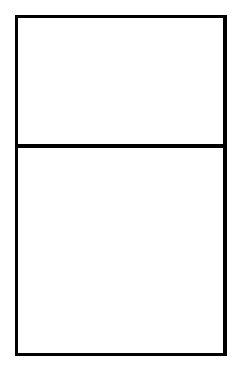
\includegraphics[width=3.5cm]{varGoldenRec}}{Rectangle d'or}
Un rectangle d'or est un rectangle dont un cot\'e vaut d'environ 1,6 fois la longueur de l'autre. Le nombre 1.6 est une approximation du ``nombre d'or''. Une belle propri\'et\'e d'un tel rectangle est que si vous coupez un carr\'e \`a l'int\'erieur du rectangle, comme le montre la figure ci-dessous, la partie gauche du rectangle est de nouveau un rectangle d'or. Vous pouvez ensuite couper un carr\'e de ce petit rectangle d'or pour en obtenir un encore plus petit, et ainsi de suite \`a l'infini. Les dimensions d'un rectangle d'or sont agr\'eables \`a l'oeil, et depuis des temps anciens, les artistes et les architectes ont utilis\'e le nombre d'or dans leurs travaux. Ecrirez un script qui dessine un rectangle d'or. Vous pouvez exprimer ce nombre en Smalltalk comme \ct{1 + 5 sqrt / 2}. 

\end{exofigwithsizeandtitle}

Expliquez pourquoi aucun des scripts qui suit n'est en mesure de dessiner une lettre A de hauteur 120 pixels. 

\begin{exonofigtitle}{Scripts ne fonctionnant pas}
\begin{code}{}
| pica hauteur |                      | pica hauteur | 
pica := Bot new.                     pica := Bot new. 
hauteur := 120.                       pica north. 
pica north.                          pica go: hauteur. 
pica go: 100.                        pica east. 
pica east.                           pica go: 70. 
pica go: 70.                         pica south. 
pica south.                          pica go: hauteur. 
pica go: 100.                        pica west. 
pica west.                           pica jump: 70. 
pica jump: 70.                       pica north. 
pica north.                          pica jump: 50. 
pica jump: 50.                       pica east. 
pica east.                           pica go: 70 
pica go: 70 	
\end{code}
\end{exonofigtitle}


\subsection{Les pyramides red\'ecouvertes}

Dans le script~\ref{scr:75}, au chapitre~\ref{cha:looping}, nous avons d\'efini le contour de la pyramide \`a pas de Saqqara comme dans le script~\ref{scr:87}.

\begin{scriptfigwithsize}[0.4]{\includegraphics[width=5cm]{varPyramid}}{La pyramide de Saqqara}\label{scr:87}
| pica | 
pica := Bot new. 
5 timesRepeat: 
[ pica north. 
pica go: 20. 
pica east. 
pica go: 20 ]. 
5 timesRepeat: 
[ pica go: 20. 
pica south. 
pica go: 20. 
pica east ]. 
pica west. 
pica go: 200.	
\end{scriptfigwithsize}


\begin{exonofigtitle}{Une pyramide avec un nombre variable de marches}\label{xp:86}
Modifiez le script~\ref{scr:75}, introduisant la variable \ct{terraceNumber} pour repr\'esenter le nombre de marches que la pyramide devrait avoir.
\end{exonofigtitle}


\begin{exonofigtitle}{Une pyramide avec un nombre variable de marches}
Modifiez le script de l'exp\'erience~\ref{xp:86} en introduisant la variable terraceSize pour repr\'esenter la taille d'une marche.
\end{exonofigtitle}


\section{Les polygones automatis\'es utilisant des variables }

L'utilisation de variables simplifie grandement la d\'efinition de scripts dans lesquels certaines \emph{variables} d\'ependent d'autres variables. Dans cette section, vous verrez comment l'utilisation de variables apporte un atout important dans le traitement des boucles. Le chapitre~\ref{cha:loopsandvariables} va plus profond\'ement dans la combinaison de variables et de boucles pouvant apparaitre dans vos programmes. 

Let us look again for a moment at Experiments~\ref{xp:73} and~\ref{xp:74}, in which a Bot was asked to 
draw a regular pentagon and a regular hexagon. The requisite code appears here as Scripts~\ref{scr:88}
and~\ref{scr:88}.

Revenons un instant sur les exp\'eriences~\ref{xp:73} et~\ref{xp:74}, dans lesquelles il a \'et\'e demand\'e \`a un Bot de dessiner un pentagone r\'egulier et un hexagone r\'egulier. Le code n\'ecessaire appara\^it ici dans les scripts~\ref{scr:88} et~\ref{scr:88}.

\begin{scriptfigwithsize}[0.4]{\includegraphics[width=3cm]{varFPentagon}}{Un pentagone r\'egulier }\label{scr:88}
| pica | 
pica := Bot new. 
5 timesRepeat: 
	[ pica go: 100. 
	pica turnLeft: 72 ] 
\end{scriptfigwithsize}

\begin{scriptfigwithsize}[0.4]{\includegraphics[width=3cm]{varFHexagon}}{Un hexagone r\'egulier }\label{scr:89}
| pica | 
pica := Bot new. 
6 timesRepeat: 
	[ pica go: 100. 
	pica turnLeft: 60 ]
\end{scriptfigwithsize}

Afin de transformer le premier script en le second script, vous devez modifier le nombre de c\^ot\'es (que nous appellerons s) \emph{et} le d\'egr\'ee de l'angle (que nous appellerons T) tel que le produit $s*T$  soit \'egal \`a 360. Ne serait-ce pas g\'enial si nous pouvions \'ecrire un script dans lequel nous aurions seulement  \`a changer un nombre unique, disons le nombre de c\^ot\'es, car c'est le param\`etre le plus simple \`a choisir? Cela peut se faire en introduisant des variables. Essayez de venir avec votre propre solution. Le script~\ref{scr:810} r\'esout le probl\`eme. Il permet de dessiner un polygone r\'egulier avec un nombre quelconque de c\^ot\'es en changeant un seul nombre. Essayez-le avant que j'en discute davantage. 

\begin{script}[810]{Dessiner un polygone r\'egulier}
| pica sides angle | 
pica := Bot new. 
sides := 6. 
angle := 360 / sides. 
sides timesRepeat: 
	[ pica go: 100. 
	pica turnLeft: angle ]
\end{script}

Ce script introduit deux nouvelles variables,  sides et angle, qui sont utilis\'es respectivement pour contenir le nombre de c\^ot\'es et la taille de l'angle. Ensuite, l'expression \ct{sides := 6}  assigne la valeur 6 \`a la variable \ct{sides}, et  l'expression \ct{angle := 360 / sides}  assigne une valeur \`a la variable angle, qui est le r\'esultat de \ct{360} divis\'e par la valeur contenue dans la variable \ct{sides}. La valeur de la variable  angle est ensuite utilis\'ee comme argument pour la commande \ct{turnLeft:} donn\'ee au robot dans le bloc \`a r\'ep\'eter.

\section{Polygones r\'eguliers avec des tailles fixes} 


Vous remarquerez que si le script~\ref{scr:810} est ex\'ecut\'e avec un grand nombre de c\^ot\'es, la figure r\'esultante ne rentre pas dans l'\'ecran. L'exp\'erience suivante vous demande de r\'esoudre ce probl\`eme en r\'eduisant la longueur des c\^ot\'es lorsque le nombre de c\^ot\'es augmente.


\begin{exofigwithsizeandtitle}[0.65]{
\includegraphics[width=3.5cm]{varSameLength}}{Contr\^oler la taille du polygone}
Modifier le script~\ref{scr:810} de mani\`ere \`a ce que la taille du polygone r\'egulier reste \`a peu pr\`es constante lorsque le nombre c\^ot\'es change. Astuce: Introduisez une variable  \ct{totalLength} qui est d\'efinie \`a une longueur fixe, et permettez \`a chaque cot\'e de votre polygone d'avoir une longueur \'egale \ct{totalLength} divis\'e par le nombre de c\^ot\'es. 


\end{exofigwithsizeandtitle}


\section{R\'esum\'e} 

\begin{itemize}
	\item Une variable est un \emph{nom} auquel on \emph{associe une valeur}. Nous devons la \emph{d\'eclarer} et lui \emph{assigner} une valeur. Ensuite, nous pouvons nous \emph{r\'ef\'erer} \`a une variable et obtenir la \emph{valeur} qui lui est associ\'ee. Il est \'egalement possible de \emph{modifier} la valeur associ\'ee \`a une variable et de lui assigner une nouvelle valeur. 

\item Une variable peut \^etre utilis\'ee partout o\`u sa valeur peut \^etre utilis\'ee.
 
\item La premi\`ere fois que nous assignons une valeur \`a une variable, nous disons que nous sommes en train de l'\emph{initialiser}.

\item Le symbole \ct{:=} assigne une valeur \`a une variable. Par exemple, \ct{hauteur := 120} assigne la valeur \ct{120} \`a la variable \ct{hauteur}, tandis que \ct{hauteur := 120 + 30} assigne le r\'esultat de l'expression \ct{120 + 30}, c'est-\`a-dire \ct{150}, \`a la variable \ct{longueur}.

\item Une variable doit g\'en\'eralement \^etre \emph{d\'eclar\'ee} et \emph{initialis\'ee} avant d'\^etre utilis\'ee. 
\end{itemize}


%%%%

% \begin{exofigwithsizeandtitle}[0.7]{\includegraphics[width=3.5cm]{}}{}
% \end{exofigwithsizeandtitle}


% \begin{script}[label]{Title.}

% \begin{figure}
% \center{\includegraphics[width=10cm]{NOTFOUND}}
% \caption{.\label{fig:}}
% \end{figure}

% \begin{exonofigtitle}{Title}
% \end{exonofigtitle}

\ifx\wholebook\relax\else
    \end{document}
\fi

%%% Local Variables:
%%% coding: utf-8
%%% mode: latex
%%% TeX-master: t
%%% TeX-PDF-mode: t
%%% ispell-local-dictionary: ``english``
%%% End: